% Number 530
% UFPM SFriction KFriction Algebra Units CAPMA
% Sliding crate on truck bed - friction
% KO

% Watermark
\AddToShipoutPicture*{\BackgroundPic}

\addtocounter {ProbNum} {1}

%\begin{floatingfigure}[r]{.45\textwidth}
%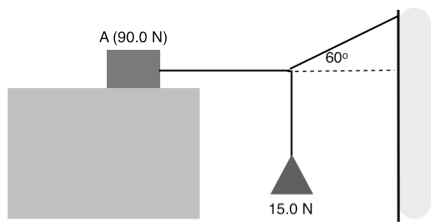
\includegraphics[scale=.6]{/Users/jgates/desktop/latex/pics/static1}
%\end{floatingfigure}
 
{\bf \Large{\arabic{ProbNum}}} A 20 kg box rests on the flat floor of a truck. The coefficients of friction between the box and floor are ${\mu_s=.15}$ and ${\mu_k=.1}$. The truck stops gently at a stop sign and then starts to move with a constant acceleration. The box is 2.2 m from the rear of the truck when the truck starts.

\bigskip
What is the maximum possible acceleration that the truck may have if the box is not to slide?

\vfill
Suppose that the acceleration of the truck is instead ${2.1~\tfrac{m}{s^2}}$. How much time elapses before the box falls off the rear of the truck? 

\vfill
How far does the truck travel in this time?

%\hfill 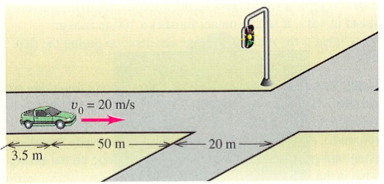
\includegraphics[scale=.85]{/Users/jgates/desktop/latex/pics/redlight.png}


\vfill
\newpage
